% プラ核講演予稿 jsarticle版
% 2段組に設定
% 以下を参照して「好ましくない表記」を解消
% % https://ichiro-maruta.blogspot.com/2013/03/latex.html
% 要件は以下の通り(年会HPによる)
% % A4縦,余白各15mm,題目は中央揃えにして1行目から,左上隅に講演番号
% 2018/12/12 T.Yokoyama@The University of Tokyo
\documentclass[a4j,11pt,twocolumn,dvipdfmx,platex]{jsarticle}
% uplatexを使用する場合は上の行をコメントアウトして以下のコメントアウトを解除
% \documentclass[a4j,11pt,twocolumn,dvipdfmx,uplatex]{jsarticle}
\usepackage[dvipdfmx]{graphicx,color}
\usepackage[T1]{fontenc}
\usepackage[margin=13.636mm]{geometry}

% スペース調整(jarticleの大きさに合わせる)
\usepackage{setspace}
\setstretch{0.9374}

\usepackage{amsmath,amssymb} %数式環境
\usepackage{bm} %数式中の太字
\usepackage{siunitx} %文章中にSI単位を記述
\usepackage[deluxe]{otf} %フォント管理

\pagestyle{empty} %ページ数を表示しない
\renewcommand{\refname}{References} %参考文献の表示を変更

\usepackage{caption}
\captionsetup[figure]{name=Fig.~,labelsep=colon}
\captionsetup[table]{name=Tbl.~,labelsep=quad}

% セクション前後の空白を調節
\makeatletter
\renewcommand{\section}{\@startsection {section}{1}{\z@}%
   {.5zh \@plus.5zh \@minus.2zh}%
   {.2zh \@plus.3zh}%
   {\normalfont\large\bfseries}%
   }
\makeatother


\begin{document}
\twocolumn[
  \noindent
  \begin{flushleft}
      \Large
      \textbf{%%%%%%%%%%%%% この下に講演番号を書いてください。%%%%%
      xPxx
      }
  \end{flushleft}
  \begin{center}
    \Large
    \textrm{%%%%%%%%%%%%% この下にタイトル(和文)を書いてください。%%%%%
    講演予稿サンプル
    }

    \textbf{    %%%%%%%%%%%%% この下にタイトル(英文)を書いてください。%%%%%
    Sample of Abstract
    }

  \vspace{1ex}

  \large \textrm{%%%%%%%%%%%%% この下に著者名(和文)を書いてください。%%%%%
  年会太郎$^1$,核融合次郎2$^2$
  }


  \textrm{%%%%%%%%%%%%% この下に著者名(英文)を書いてください。%%%%%
  Taro Nenkai$^1$, Jiro Kakuyugo$^2$,
  }

  \vspace{1ex}


  \textrm{%%%%%%%%%%%%% この下に所属(和文)を書いてください。%%%%%
  プラズマ大学$^1$,某研究所$^2$
  }

  \textrm{%%%%%%%%%%%%% この下に所属(英文)を書いてください。%%%%%
  Plasma University$^1$, Nanigashi Institute$^2$
  }

  \end{center}
  \normalsize

  \vspace{1ex}
]

%%%%%%%%%%%%% この下に本文を書いてください。%%%%%
\section{本文}
\label{sec:本文}
これはプラズマ核融合学会年会の講演予稿サンプルです.
予稿本文をここに記述します.
A4縦2段組みです.

\begin{figure}[h]
  \centering
  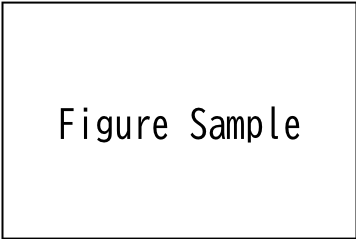
\includegraphics{fig.png}
  \caption{図のサンプル.}
  \label{fig:figure_label}
\end{figure}

数式のサンプル(式\ref{eq:sample}).

\begin{align}
  \nabla P = j \times B
  \label{eq:sample}
\end{align}

%%%%%%%%%%%%% この下に参考文献を書いてください。%%%%%
%\footnotesize
%\bibliographystyle{unsrt_short}
%\bibliography{bibfile}

\end{document}
